\section{Functionality}
In this section, we describe the main features and functionality of the Safety Annex.
%
An AADL model of the nominal system behavior specifies the hardware and software components of the system and their interconnections. This nominal model is then annotated with assume-guarantee contracts using the AGREE annex~\cite{NFM2012:CoGaMiWhLaLu} for AADL. The nominal model  requirements are verified using compositional verification techniques based on $k$-induction model checking~\cite{2017arXiv171201222G}.

Once the nominal model behavior is defined and verified, the Safety Annex can be used to specify possible faulty behaviors for each component. The faults are defined on each of the relevant components using a customizable library of fault nodes and the faults are assigned a probability of occurrence. A probability threshold is also defined at the system level. This extended model can be analyzed to verify the behavior of the system in the presence of faults. Verification of the nominal model with or without the fault model is controlled through the safety analysis option during AGREE verification.

To illustrate the syntax of the Safety Annex, we use an example based on the Wheel Brake System (WBS) described in ~\cite{AIR6110} and used in our previous work ~\cite{Stewart17:IMBSA}.
The fault library contains commonly used fault node definitions. An example of a fault node is shown below:
\begin{figure}[h!]
\vspace{-0.19in}
\begin{center}
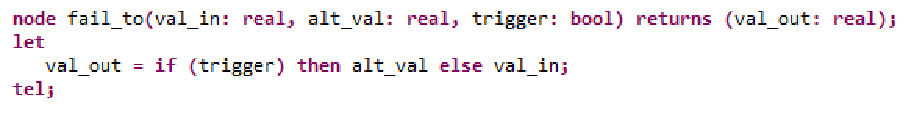
\includegraphics[trim=0 9 0 5,clip,width=1.0\textwidth]{images/faultNode.png}
\end{center}
\vspace{-0.4in}
\end{figure}

The \textit{fail\_to} node provides a way to inject a faulty input value. When the \textit{trigger} condition is satisfied, the nominal component output value is overridden by the \textit{fail\_to} failure value. In the WBS, the pump component generates an expected amount of pressure to a hydraulic line.  Declaration of a non-deterministic fault in the pump component is shown below:
\begin{figure}[h!]
\vspace{-0.17in}
\begin{center}
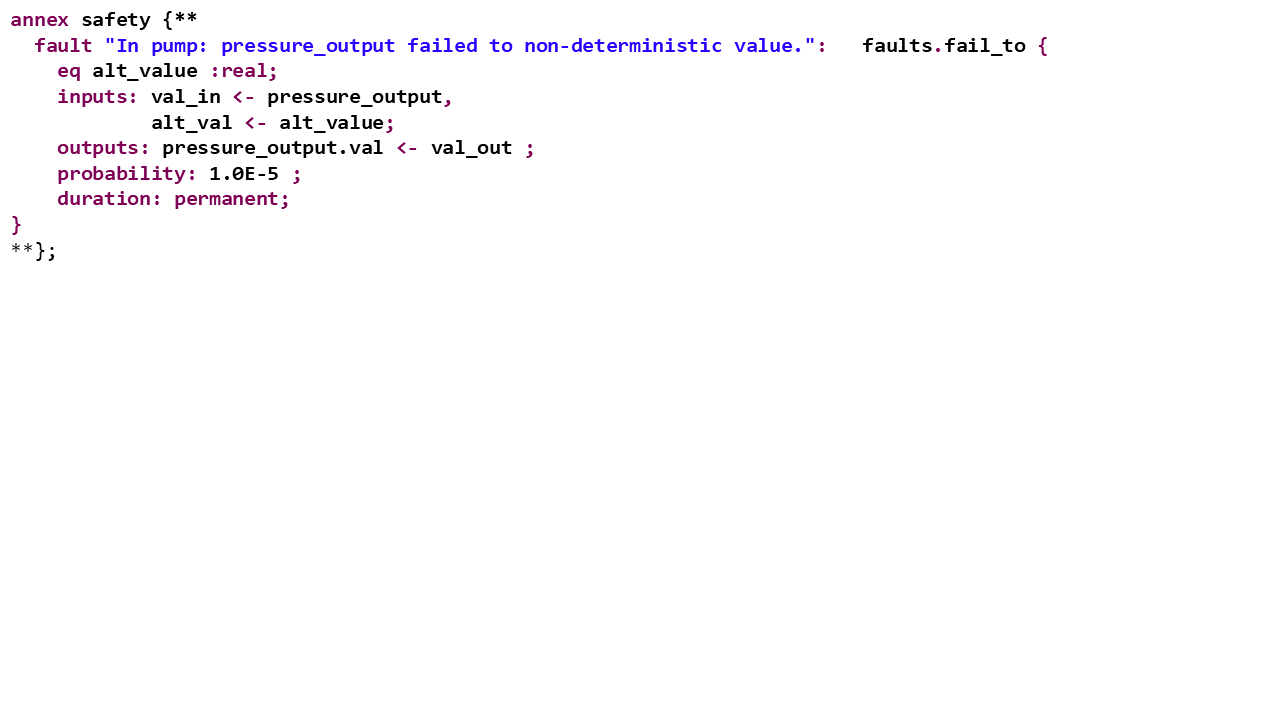
\includegraphics[trim=0 330 150 0,clip,width=1.0\textwidth]{images/annex.png}
\end{center}
\vspace{-0.40in}
\end{figure}

The \textit{fault statement} consists of a unique description string, the fault node definition name, and a series of \textit{fault subcomponent} statements. \\
\textbf{Inputs} in a fault statement are the parameters of the fault node definition. In the example above, \textit{val\_in} and \textit{alt\_val} are the two input parameters of the fault node. These are linked to the output from the Pump component (\textit{pressure\_output.val}), and \textit{alt\_value}, a nondeterministic value defined within the Safety Annex. When the analysis is run, these values are passed into the fault node definition.\\
\textbf{Outputs} of the fault definition correspond to the outputs of the fault node. The fault output statement links the component output (\textit{pressure\_output.val}) with the fault node output (\textit{val\_out}). If the fault is triggered, the nominal value of \textit{pressure\_output.val} is overridden by the failure value output by the fault node. Faulty outputs can take deterministic or non-deterministic values. \\
\textbf{Probability} (optional) describes the probability of a fault occurrence.\\
\textbf{Duration} describes the duration of the fault; currently the Safety Annex supports transient and permanent faults.\\
%\textit{Equation Statements}: Equation statements support deterministic or nondeterministic types. For more details on equation statements, see ~\cite{NFM2012:CoGaMiWhLaLu}.





